%\documentclass[a4paper,fleqn,longmktitle]{cas-sc}
\documentclass[a4paper,fleqn]{cas-sc}

%\usepackage[numbers]{natbib}
%\usepackage[authoryear]{natbib}
\usepackage[authoryear,longnamesfirst]{natbib}

\usepackage{float}
\usepackage{subcaption}
\usepackage{caption}
\usepackage[table]{xcolor}

%%%Author macros
\def\tsc#1{\csdef{#1}{\textsc{\lowercase{#1}}\xspace}}
\tsc{WGM}
\tsc{QE}
\tsc{EP}
\tsc{PMS}
\tsc{BEC}
\tsc{DE}
%%%
%comentario teste para ver o git
\begin{document}
	\let\WriteBookmarks\relax
	\def\floatpagepagefraction{1}
	\def\textpagefraction{.001}
	\shorttitle{Neural TCP}
	\shortauthors{J.K. Krishnan et~al.}
	%\begin{frontmatter}
	
	\title [mode = title]{This is a specimen $a_b$ title}                      
	\tnotemark[1,2]
	
	\tnotetext[1]{This document is the results of the research
		project funded by the National Science Foundation.}
	
	\tnotetext[2]{The second title footnote which is a longer text matter
		to fill through the whole text width and overflow into
		another line in the footnotes area of the first page.}
	
	
	\author[1,3]{J.K. Krishnan}[type=editor,
	auid=000,bioid=1,
	prefix=Sir,
	role=Researcher,
	orcid=0000-0001-0000-0000]
	\cormark[1]
	\fnmark[1]
	\ead{jkk@example.in}
	\ead[url]{www.jkkrishnan.in}
	
	\credit{Conceptualization of this study, Methodology, Software}
	
	\affiliation[1]{organization={Department of Physics, J.K. Institute of Science},
		addressline={Jawahar Nagar}, 
		city={Trivandrum},
		%               citysep={}, % Uncomment if no comma needed between city and postcode
		postcode={695013}, 
		state={Kerala},
		country={India}}
	
	\author[2,4]{Han Thane}[style=chinese]
	
	\author[2,3]{William {J. Hansen}}[%
	role=Co-ordinator,
	suffix=Jr,
	]
	\fnmark[2]
	\ead{wjh@example.org}
	\ead[URL]{https://www.university.org}
	
	\credit{Data curation, Writing - Original draft preparation}
	
	\affiliation[2]{organization={World Scientific University},
		addressline={Street 29}, 
		postcode={1011 NX}, 
		postcodesep={}, 
		city={Amsterdam},
		country={The Netherlands}}
	
	\author[1,3]{T. Rafeeq}
	\cormark[2]
	\fnmark[1,3]
	\ead{t.rafeeq@example.in}
	\ead[URL]{www.campus.in}
	
	\affiliation[3]{organization={University of Intelligent Studies},
		addressline={Street 15}, 
		city={Jabaldesh},
		postcode={825001}, 
		state={Orissa}, 
		country={India}}
	
	\cortext[cor1]{Corresponding author}
	\cortext[cor2]{Principal corresponding author}
	\fntext[fn1]{This is the first author footnote, but is common to third
		author as well.}
	\fntext[fn2]{Another author footnote, this is a very long footnote and
		it should be a really long footnote. But this footnote is not yet
		sufficiently long enough to make two lines of footnote text.}
	
	\nonumnote{This note has no numbers. In this work we demonstrate $a_b$
		the formation Y\_1 of a new type of polariton on the interface
		between a cuprous oxide slab and a polystyrene micro-sphere placed
		on the slab.
	}
	
	\begin{abstract}
		The advancement and ubiquity of digital networks have fundamentally transformed numerous spheres of human activity. At the heart of this phenomenon, lies the Transmission Control Protocol (TCP) model, whose influence is particularly notable in the exponential growth of the Internet due to its ability to transmit flexibly to any device, through its advanced Congestion Control (CC). Seeking an even more efficient CC mechanism, this work proposes the construction of deep learning neural networks (MLP, LSTM, and CNN) for classifying the level of network congestion. The results attest to models capable of distinguishing, with over 90\% accuracy, between moments of high and low degrees of congestion. With this, it becomes possible to differentiate between congestion and random losses, potentially increasing throughput by up to five times in environments with random losses when combined with CC algorithms.
		
		\noindent\texttt{\textbackslash begin{abstract}} \dots 
		\texttt{\textbackslash end{abstract}} and
		\verb+\begin{keyword}+ \verb+...+ \verb+\end{keyword}+ 
		which
		contain the abstract and keywords respectively. 
		Each keyword shall be separated by a \verb+\sep+ command.
	\end{abstract}
	
	\begin{graphicalabstract}
		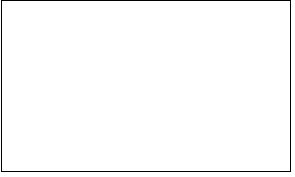
\includegraphics{figs/cas-grabs.pdf}
	\end{graphicalabstract}
	
	\begin{highlights}
		\item Research highlights item 1
		\item Research highlights item 2
		\item Research highlights item 3
	\end{highlights}
	
	\begin{keywords}
		quadrupole exciton \sep polariton \sep \WGM \sep \BEC
	\end{keywords}
	
	
	\maketitle

\centering
\begin{figure}[!htb]
	\begin{minipage}{0.45\textwidth}
	\begin{subfigure}[t]{0.25\textwidth}
		\centering
		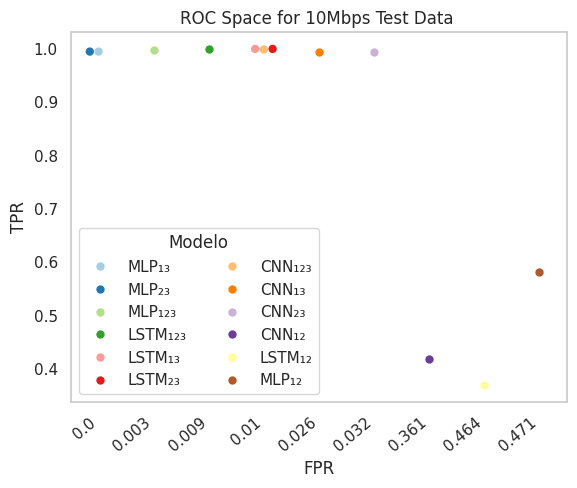
\includegraphics[width=1.0\textwidth]{./figs/ROC-Space-Test-Data-10Mbps.png}
		\caption{Lorem ipsum}
	\end{subfigure}%
	~ 
	\begin{subfigure}[t]{0.25\textwidth}
		\centering
		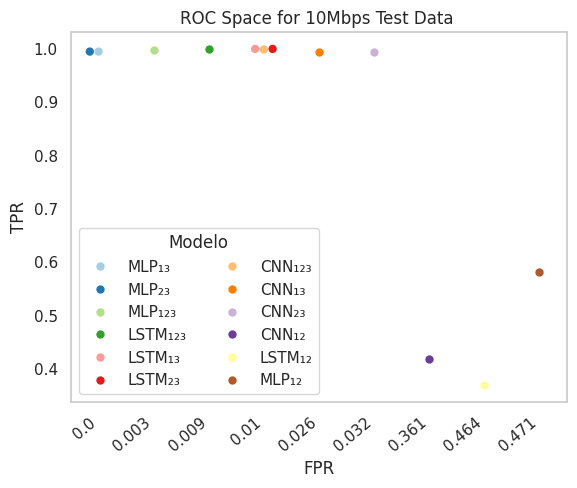
\includegraphics[width=1.0\textwidth]{./figs/ROC-Space-Test-Data-10Mbps.png}
		\caption{Lorem ipsum, lorem ipsum,Lorem ipsum, lorem ipsum,Lorem ipsum}
	\end{subfigure}
	\caption{Caption place holder}
\end{minipage}
\end{figure}


\end{document}